\documentclass[12pt, letterpaper]{article}
\usepackage{geometry}
\usepackage[T1]{fontenc}
\usepackage[utf8]{inputenc}
\usepackage[english,russian]{babel}
\usepackage{titlesec}
\usepackage{graphicx}
\usepackage{xcolor}
\usepackage{framed}
\usepackage{booktabs}
\usepackage{wrapfig}
\usepackage{pgfplots}
\usepackage{listings}
\lstset{
    basicstyle=\ttfamily\small, % Моноширинный шрифт
    keywordstyle=\color{blue},   % Ключевые слова синие
    commentstyle=\color{green},  % Комментарии зеленые
    stringstyle=\color{red},     % Строки красные
    numbers=left,               % Нумерация строк слева
    identifierstyle=\color{black},
    numberstyle=\tiny\color{gray}, % Стиль номеров строк
    frame=single,               % Рамка вокруг кода
    frameround=tttt,
    showstringspaces=false,
    backgroundcolor=\color{gray!10},
    breaklines=true,            % Перенос длинных строк
    tabsize=4                   % Размер табуляции
}
\titleformat{\section}{\bfseries\large}{\thesection}{0.5em}{}
\geometry{
    a4paper,
    left = 2cm,
    right = 2cm,
    top = 2cm,
    bottom = 2cm
}

\begin{document}
    \begin{titlepage}
        \begin{center}
            \large\textbf{МОСКОВСКИЙ ФИЗИКО-ТЕХНИЧЕСКИЙ ИНСТИТУТ (НАЦИОНАЛЬНЫЙ ИССЛЕДОВАТЕЛЬСКИЙ УНИВЕРСИТЕТ)}\\
            \large\textbf{Физтех-школа Радиотехники и компьютерных технологий}\\
            \vspace{8cm}
            \Large\textbf{Лабораторная работа}\\
            \large{Исследование зависимости времени выполнения программы от уровня оптимизации}\\
            \vspace{5cm}
        \end{center}
        \begin{flushright}
            \large\textbf{Выполнил:}\\
            \large{Рогов Анатолий}\\
            \large{Б01-406}\\
        \end{flushright}
        \begin{center}
            \vfill
            \large\textbf{г. Долгопрудный}\\
            \large\textbf{\the \year}\\
        \end{center}
    \end{titlepage}

    \paragraph{Цель работы:}1) построение модели множества Мандельброта с различными способами вычисления; 2) измерение времени выполнения программы с каждым из способов и проанализировать исследуемую зависимость.
    \paragraph{В работе используются:}графическая библиотека SFMl 2.6.1, библиотека time, библиотека immintrin.\\

    Во многих случаях скорость выполнения программы является очень важным фактором при её разработке. Если программа должна обрабатывать видеокадры или сетевые пакеты в масштабе реального времени, то медленно работающая программа не сможет обеспечить необходимую функциональность. Посмотрим, как можно ускорить работу программ с помощью нескольких приемов оптимизации.

    Чтобы написать эффективную программу, необходимо, во-первых, подобрать наилучший набор алгоритмов и структур данных и, во-вторых, написать код, который компилятор сможет превратить в эффективный выполняемый код. Внешне незначительные изменения в исходном коде программы могут радикально повлиять на успех ее оптимизации компилятором. В-третьих (это особенно касается преимущественно вычислительных задач), необходимо разделить задачи на части, которые можно вычислять параллельно, используя преимущества многоядерных и многопроцессорных систем.

    Первый шаг в оптимизации программы – устранение ненужной работы, чтобы код выполнял намеченную задачу с максимальной эффективностью. Под этим подразумевается устранение ненужных вызовов функций, условных проверок и обращений к памяти. Эти оптимизации не зависят от каких-либо конкретных свойств целевой машины.

    Понимая, как работает процессор, мы сможем сделать второй шаг в оптимизации программы и использовать способность процессоров выполнять несколько инструкций параллельно.

    В данной работе оптимизация кода по построению множества Мандельброта выглядит простым и линейным процессом применения серии преобразований в определенном порядке. Основные версии функции по построению множества:

    1. Базовая версия - непосредственные арифметические преобразования для каждой отдельной точки;

    2-3. Версия на массивах - представление точек в виде последовательностей из 4 элементов с применением арифметических операций для каждой из них.

    4. Intrinsics версия - применение встроенных возможностей процессора для полной векторизации вычислений.

    \subparagraph{Множество Мандельброта.}
    Множество Мандельброта — это фрактальное множество на комплексной плоскости, которое определяется простой итерационной формулой, но демонстрирует чрезвычайно сложную и красивую структуру. Оно было впервые описано Бенуа Мандельбротом в 1980 году и стало одним из самых известных примеров математических фракталов.

    Множество Мандельброта строится на основе итераций комплексного квадратичного отображения: $z_{n+1} = z_{n}^2 + c$, где:
    $z$ — комплексная переменная (начальное значение $z_0 = 0$), $c$ — комплексная константа (параметр, определяющий точку на плоскости).

    Правило принадлежности:\\
    Точка $c$ принадлежит множеству Мандельброта, если последовательность $z_n$ не стремится к бесконечности при $n \to \infty$. На практике итерации выполняют до определённого предела (например, $n_{max} = 1000$), и если $\left| z_n \right|$ остаётся меньше некоторого порога (обычно 2), то $c$ считается принадлежащей множеству.

    \subparagraph{Intrinsics functions.}
    Интринсики (intrinsics) — это специальные функции или конструкции которые предоставляют низкоуровневый доступ к возможностям процессора, минуя стандартные механизмы компилятора. Они используются для оптимизации критически важных участков кода, где важны производительность и контроль над аппаратными ресурсами. Использование SIMD-инструкций (AVX, SSE, SIMD) позволяет выполнять одну операцию над несколькими данными одновременно (векторизация), например, обработка изображений и физические расчеты.

    \paragraph{Ход работы}
    Измерим приборную погрешность:\\
    \begin{wraptable}{l}{0.25\textwidth}
        \begin{tabular}{cc}
        \toprule             % верхняя линия
        \textbf{№} & \textbf{Время t, c} \\
        \midrule             % разделитель заголовка
        1 & 0,0061 \\
        2 & 0,0072 \\
        3 & 0,0080 \\
        4 & 0,0076 \\
        5 & 0,0059 \\
        6 & 0,0036 \\
        7 & 0,0064 \\
        8 & 0,0035 \\
        9 & 0,0049 \\
        10 & 0,0033 \\
        \bottomrule          % нижняя линия
        \end{tabular}
    \end{wraptable}

    \begin{lstlisting}[language=C]
    #include <stdio.h>
    #include <time.h>

    int main(int argc, char* argv[]) {
        printf("PROGRAM TIME: %lg sec\n", (double)clock() / CLOCKS_PER_SEC);
        return 0;
    }
    \end{lstlisting}

    $\bar{t} = 0,0057$ с\\

    $\sigma = 8,6 \cdot 10^{-6}$ с\\

    $\epsilon = 0,15\%$

    \begin{wraptable}{l}{1\textwidth}
    Для проверки правильности применения соответствующих оптимизаций будем сравнивать результаты вычислений множества Мандельброта с помощью графической библиотеки. Будем следить за изменениями полученного изображения, чтобы исправить оптимизации, нарушившие ход выполнения программы. Все последующие измерения времени будем проводить без использовани графической библиотеки, рассчитывая каждую из точек по 300 раз. Окончательный результат поделим на 300 для получения времени на рассчет одной точки.

    \section{Базовая версия} (MandelbrotStatusCode BaseVersionMandelbrot(SFML* sfml, Mandel\_struct* mnd))

    \end{wraptable}

    \begin{figure}[h]
        \centering
        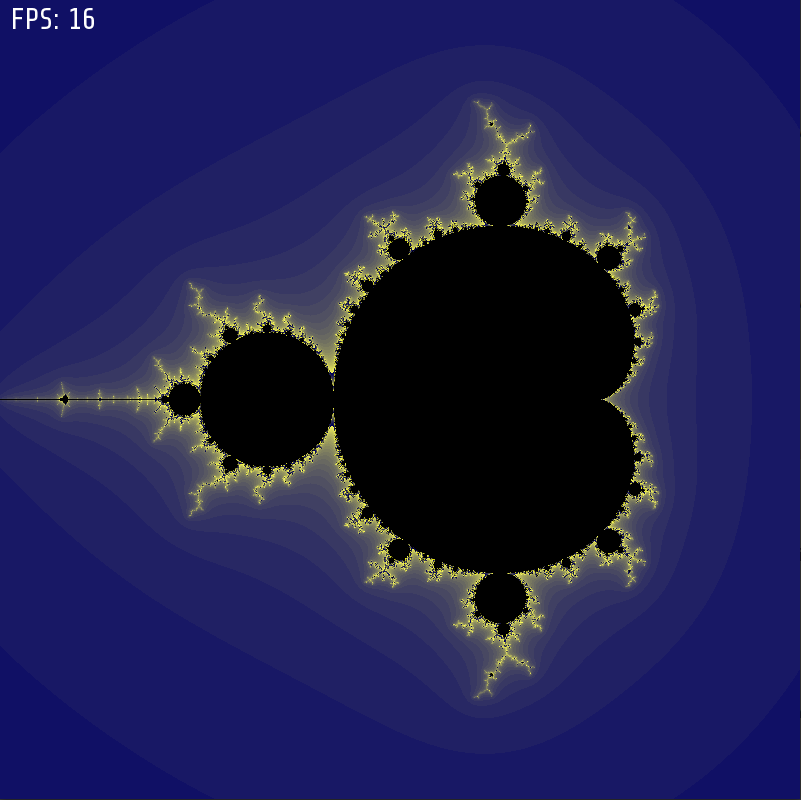
\includegraphics[width=0.4\linewidth]{../data/imgs/mandelbrot.png}
        \caption{Базовая версия Мандельброта}
        \label{fig:enter-label}
    \end{figure}

    \begin{wraptable}{l}{0.5\textwidth}
        \begin{tabular}{cc}
        \toprule             % верхняя линия
        \textbf{№} & \textbf{Время t, c} \\
        \midrule             % разделитель заголовка
        1 & 18,8060 \\
        2 & 18,7392 \\
        3 & 18,7976 \\
        4 & 18,7988 \\
        5 & 18,7220 \\
        6 & 18,8098 \\
        7 & 18,7519 \\
        8 & 18,8037 \\
        9 & 18,8196 \\
        10 & 18,7322 \\
        \bottomrule          % нижняя линия
        \end{tabular}
    \end{wraptable}

     С оптимизацией -O3:\\

    $\bar{t} = 18,7781 (0,0626)$ с\\

    $\sigma = 2,9 \cdot 10^{-2}$ с\\

    $\epsilon = 0,15\%$\\

    $\bar{FPS} = 16,86$\\

    $\sigma = 0,16$\\

    $\epsilon = 0,96\%$\\

    \begin{wraptable}{l}{0.5\textwidth}
        \begin{tabular}{cc}
        \toprule             % верхняя линия
        \textbf{№} & \textbf{Время t, c} \\
        \midrule             % разделитель заголовка
        1 & 39,7885 \\
        2 & 39,7820 \\
        3 & 39,8798 \\
        4 & 39,7425 \\
        5 & 40,0279 \\
        6 & 39,8741 \\
        7 & 39,5767 \\
        8 & 39,5836 \\
        9 & 39,5924 \\
        10 & 39,6434 \\
        \bottomrule          % нижняя линия
        \end{tabular}
    \end{wraptable}

    Без оптимизации -O3:\\

    $\bar{t} = 39,7491 (0,1325)$ с\\

    $\sigma = 8,9 \cdot 10^{-2}$ с\\

    $\epsilon = 0,22\%$\\

    $\bar{FPS} = 8,46$\\

    $\sigma = 0,02$\\

    $\epsilon = 0,3\%$\\

    \newpage
    \section{Версия на массивах} (MandelbrotStatusCode ArrayVersionMandelbrot(SFML* sfml, Mandel\_struct* mnd))

    \begin{wraptable}{l}{0.5\textwidth}
        \begin{tabular}{cc}
        \toprule             % верхняя линия
        \textbf{№} & \textbf{Время t, c} \\
        \midrule             % разделитель заголовка
        1 & 10,0406 \\
        2 & 10,4789 \\
        3 & 10,1374 \\
        4 & 10,4909 \\
        5 & 10,1487 \\
        6 & 10,5347 \\
        7 & 10,0543 \\
        8 & 10,0491 \\
        9 & 10,5100 \\
        10 & 10,1447 \\
        \bottomrule          % нижняя линия
        \end{tabular}
    \end{wraptable}

     С оптимизацией -O3:\\

    $\bar{t} = 10,2589 (0,0342)$ с\\

    $\sigma = 13,21 \cdot 10^{-2}$ с\\

    $\epsilon = 1,3\%$\\

    $\bar{FPS} = 29,12$\\

    $\sigma = 0,94$\\

    $\epsilon = 3,2\%$\\

    \begin{wraptable}{l}{0.5\textwidth}
        \begin{tabular}{cc}
        \toprule             % верхняя линия
        \textbf{№} & \textbf{Время t, c} \\
        \midrule             % разделитель заголовка
        1 & 255,335 \\
        2 & 255,162 \\
        3 & 255,003 \\
        4 & 254,834 \\
        5 & 254,654 \\
        \bottomrule          % нижняя линия
        \end{tabular}
    \end{wraptable}
    Без оптимизации -O3:\\
    $\bar{t} = 254,99 (0,8499)$ с\\
    $\sigma = 41,00 \cdot 10^{-2}$ с\\
    $\epsilon = 0,16\%$\\
    $\bar{FPS} = 1,7653$\\
    $\sigma = 0,0004$\\
    $\epsilon = 0,03\%$\\

    \begin{wraptable}{l}{1\textwidth}
    \section{Интринсик версия} (MandelbrotStatusCode IntrinsicsVersionMandelbrot(SFML* sfml, Mandel\_struct* mnd))
    \end{wraptable}

    \begin{wraptable}{l}{0.5\textwidth}
        \begin{tabular}{cc}
        \toprule             % верхняя линия
        \textbf{№} & \textbf{Время t, c} \\
        \midrule             % разделитель заголовка
        1 & 6,2255 \\
        2 & 6,1537 \\
        3 & 6,1791 \\
        4 & 6,1784 \\
        5 & 6,2339 \\
        6 & 6,1735 \\
        7 & 6,1968 \\
        8 & 6,1878 \\
        9 & 6,1913 \\
        10 & 6,1833 \\
        \bottomrule          % нижняя линия
        \end{tabular}
    \end{wraptable}

     С оптимизацией -O3:\\

    $\bar{t} = 6,1903 (0,02063)$ с\\

    $\sigma = 0,9 \cdot 10^{-2}$ с\\

    $\epsilon = 0,15\%$\\

    $\bar{FPS} = 47,35$\\

    $\sigma = 4,23$\\

    $\epsilon = 8,9\%$\\

    \newpage
    \begin{wraptable}{l}{0.5\textwidth}
        \begin{tabular}{cc}
        \toprule             % верхняя линия
        \textbf{№} & \textbf{Время t, c} \\
        \midrule             % разделитель заголовка
        1 & 32,1174 \\
        2 & 31,8332 \\
        3 & 32,1725 \\
        4 & 32,2244 \\
        5 & 32,1574 \\
        6 & 32,1550 \\
        7 & 31,9391 \\
        8 & 32,1791 \\
        9 & 32,1090 \\
        10 & 31,8814 \\
        \bottomrule          % нижняя линия
        \end{tabular}
    \end{wraptable}

    Без оптимизации -O3:\\

    $\bar{t} = 32,0769 (0,1069)$ с\\

    $\sigma = 7,3 \cdot 10^{-2}$ с\\

    $\epsilon = 0,23\%$\\

    $\bar{FPS} = 10,17$\\

    $\sigma = 0,01$\\

    $\epsilon = 0,9\%$\\

    \paragraph{Анализ результатов}

    В силу значительных отличий результатов измерения времени для vector (array) версии опустим её значения на итоговой гистограмме:

    \begin{figure}[h]
        \centering
        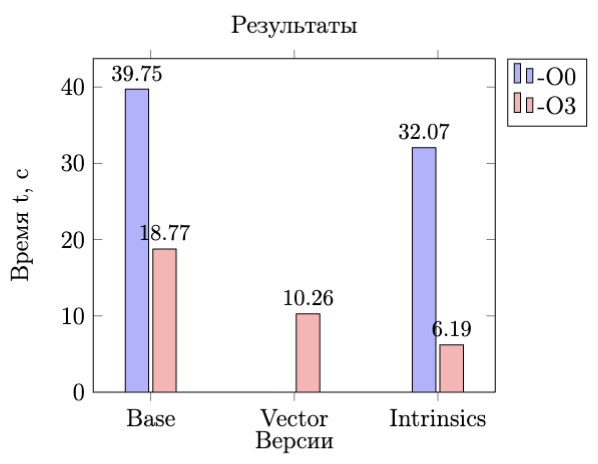
\includegraphics[width=0.7\linewidth]{../data/imgs/results.png}
        \label{fig:enter-label}
    \end{figure}

    \paragraph{Вывод:}
    Я воссоздал математическую модель множества Мандельброта с помощью графической библиотеки SFML 2.6.1. Измерил время выполнения программы на каждом из уровней оптимизации. Итоговый прирост оптимизаций, проделанных в работе, составляет: $\frac{18.78}{6.19} \approx 3$. Полученный результат попадает в диапазон ожидаемых значений для оптимизаций без применения многопоточности!

\end{document}
